\begin{mainquestion}{transformerpowertransfer}{Ideal Transformer Power}

Consider the ideal transformer circuit shown below.

\begin{center}
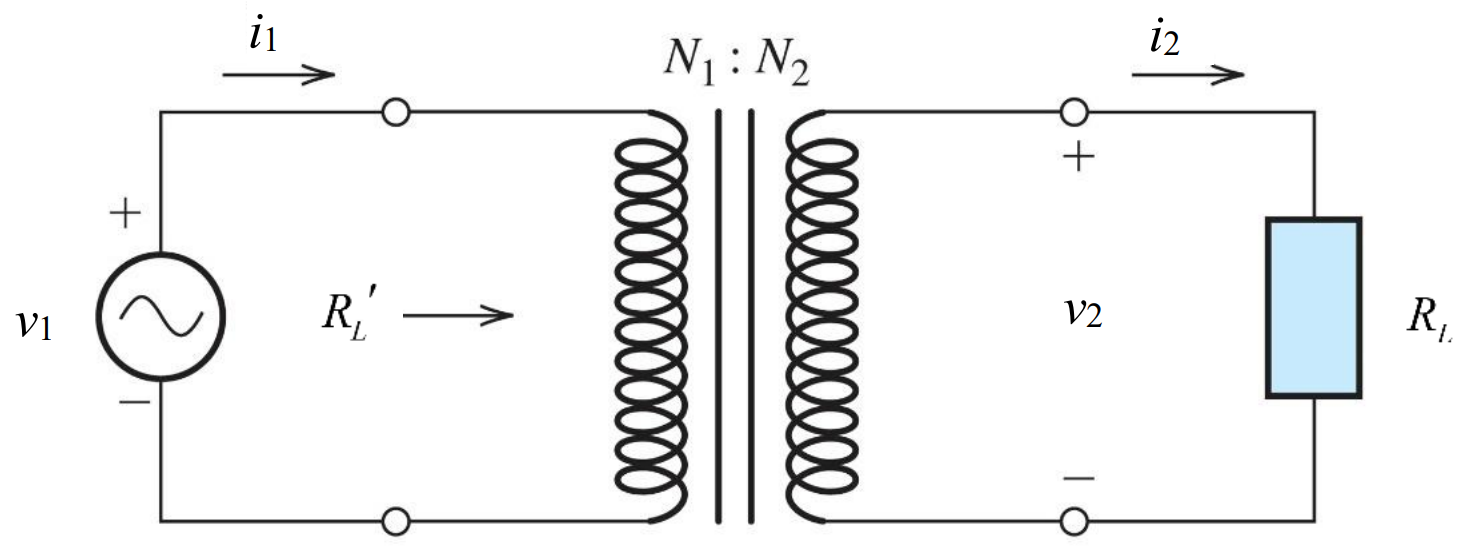
\includegraphics[width=0.9\textwidth]{xfor_basic.png}
\end{center}

% =========================================================
\begin{partquestion}{resistancetransformation}
{Derive the resistance $R_L' = v_1 / i_1$ seen by the source, assuming an ideal transformer. This is a simple \emph{resistance transformation} across the transformer.}

\begin{answer}
For an ideal transformer:
\[
\frac{v_2}{v_1} = \frac{N_2}{N_1} \quad \text{and} \quad \frac{i_2}{i_1} = \frac{N_1}{N_2}
\]

It is straightforward to show that:

\[
R_L' \equiv \frac{v_1}{i_1} = \frac{v_2(N_1/N_2)}{i_2(N_2/N_1)} = \frac{v_2}{i_2}\left(\frac{N_1}{N_2}\right)^2 = R_L\left(\frac{N_1}{N_2}\right)^2
\]

The resistance as seen from the primary side is scaled by the square of the turns ratio.
\end{answer}
\end{partquestion}

% =========================================================
\begin{partquestion}{directtransmission}
{Consider a 10 V peak-to-peak sinusoidal source connected to a resistive load of 17 $\Omega$ via a transmission line without transformers, having a total line resistance of 17 $\Omega$. Determine the power delivered by the source, the power dissipated in the line, the power delivered to the load, and the efficiency $\eta = P_{\text{load}} / P_{\text{source}} \times 100\%$.}

\begin{center}
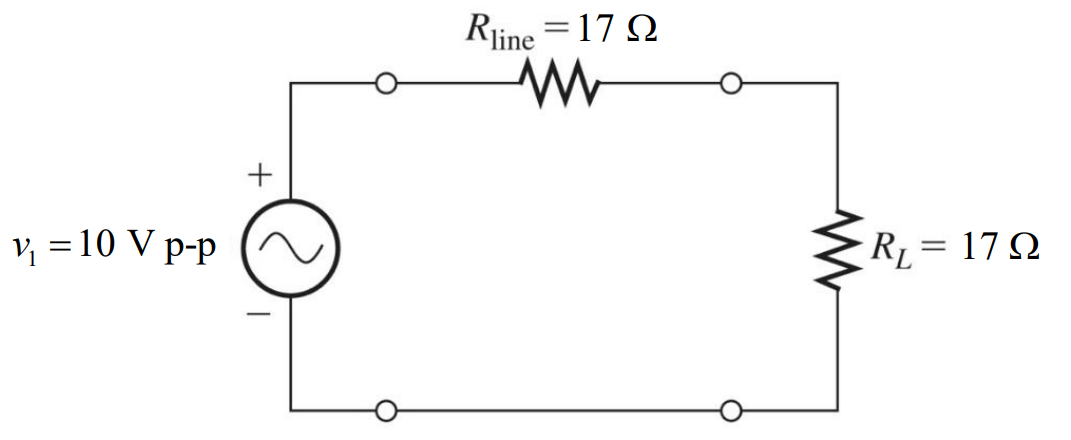
\includegraphics[width=0.9\textwidth]{no_xfor.png}
\end{center}

\begin{answer}
The power delivered by the source is $P = v_{1,\text{rms}}^2 / (R_{\text{line}} + R_L)$. The voltage is given as peak-to-peak, so the amplitude is 5~V and the RMS value is $5/\sqrt{2}$~V.

\[
P_{\text{delivered}} = \frac{v_{1,\text{rms}}^2}{R_{\text{line}} + R_L} = \frac{(5/\sqrt{2})^2}{17 + 17} = \frac{25}{2(34)} \approx 368\text{ mW}
\]

The power dissipated in the line is:

\[
P_{\text{line}} = \frac{v_{\text{line,rms}}^2}{R_{\text{line}}} = \left(\frac{R_{\text{line}}}{R_{\text{line}} + R_L} v_{1,\text{rms}}\right)^2 \frac{1}{R_{\text{line}}} = \left(\frac{17}{34} \cdot \frac{5}{\sqrt{2}}\right)^2 \frac{1}{17} = \frac{25}{8 \cdot 17} = 184\text{ mW}
\]

The remaining power is dissipated in the load:

\[
P_{\text{load}} = 368\text{ mW} - 184\text{ mW} = 184\text{ mW}
\]

The efficiency is:

\[
\eta = \frac{184\text{ mW}}{368\text{ mW}} \times 100\% = 50\%
\]

This circuit delivers maximum power transfer to the load because line resistance is equal to that of the source resistance.
\end{answer}
\end{partquestion}

% =========================================================
\begin{partquestion}{withstepuptransformers}
{Now introduce a pair of transformers: a step-up transformer (1:10) before the transmission line and a step-down transformer (10:1) after the transmission line, as shown below. Using the result from part (\cref{prob:transformerpowertransfer:resistancetransformation}), transform the resistance to the source side of the transformer and again determine the power delivered by the source, the power dissipated in the line, the power delivered to the load, and the efficiency. Is this circuit delivering maximum power transfer to the load (which in this case occurs when the load resistance when transformed across the step-down transformer is equal to the line resistance)?}

\begin{center}
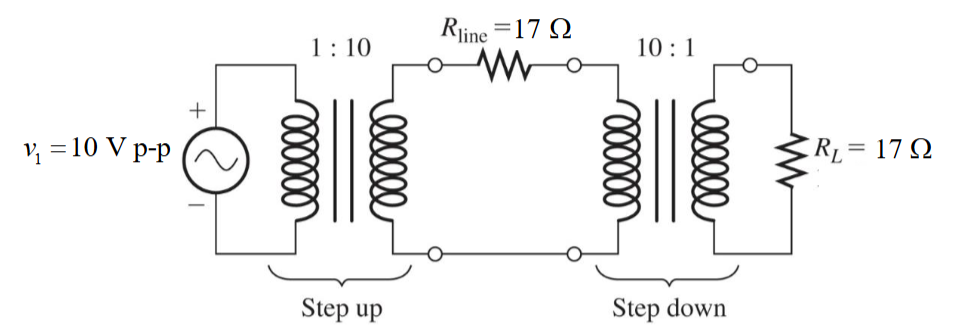
\includegraphics[width=0.9\textwidth]{with_xfor.png}
\end{center}

\begin{answer}
The load needs to be transformed across the step-down transformer, and then both resistors need to be transformed across the step-up transformer.

First resistance transformation (load across step-down transformer):

\[
R_L'' = R_L \left(\frac{10}{1}\right)^2 = 100 R_L = 1700\text{ }\Omega
\]

Second resistance transformation (both resistors across step-up transformer):

\[
R_L' = \left(R_{\text{line}} + R_L''\right) \left(\frac{1}{10}\right)^2 = \frac{R_{\text{line}}}{100} + R_L = \frac{17}{100} + 17 = 17.17\text{ }\Omega
\]

The power delivered is:

\[
P_{\text{delivered}} = \frac{(5/\sqrt{2})^2}{0.17 + 17} = \frac{25}{2(17.17)} \approx 728\text{ mW}
\]

The power dissipated in the line (which now sees voltage stepped up by factor of 10):

\[
P_{\text{line}} = \frac{[v_{1,\text{rms}} \cdot \frac{R_{\text{line}}/100}{ R_{\text{line}}/100 + R_L}]^2}{R_{\text{line}}/100} = \frac{(\frac{5}{\sqrt{2}})^2(17/100)}{(17/100 + 17)^2} \approx 7.2\text{ mW}
\]

The remaining power is dissipated in the load:

\[
P_{\text{load}} = 728\text{ mW} - 7.2\text{ mW} = 721\text{ mW}
\]

The efficiency is:

\[
\eta = \frac{721\text{ mW}}{728\text{ mW}} \times 100\% = 99\%
\]

This circuit is \textbf{not} delivering maximum power transfer to the load because the line resistance is not equal to that of the (transformed) load
resistance.
\end{answer}
\end{partquestion}

% =========================================================
\begin{partquestion}{comparisonimplications}
{Comparing answers to parts (\cref{prob:transformerpowertransfer:directtransmission}) and (\cref{prob:transformerpowertransfer:withstepuptransformers}), what do your results indicate?}

\begin{answer}
The use of a transformer pair to step up and step down the voltage provides a much more efficient mechanism to transport power over transmission lines. The efficiency improved from 50\% to 99\% by using transformers to step up voltage before transmission and step down after. Note that greater efficiency does not imply that the maximum power is being transferred!
\end{answer}
\end{partquestion}

% =========================================================
\begin{partquestion}{dcsource}
{Will your results be the same in parts (\cref{prob:transformerpowertransfer:directtransmission}) and (\cref{prob:transformerpowertransfer:withstepuptransformers}) if the source is replaced by a 10 V DC battery? What about the efficiency? Explain your answers.}

\begin{answer}
For part (\cref{prob:transformerpowertransfer:directtransmission}), not quite, since the original AC voltage source was 10 V peak-to-peak. An equivalent DC battery from a power perspective would be one operating at $5/\sqrt{2} \approx 3.54$~V.

For part (\cref{prob:transformerpowertransfer:withstepuptransformers}), not at all, because transformers block all DC voltages from propagating down the transmission line. There will be no power dissipated in the load (or the line!).
\end{answer}
\end{partquestion}

\end{mainquestion}
